\documentclass{article}
\usepackage[margin = 0.5in]{geometry}
\usepackage[table]{xcolor}
\usepackage{amsmath,amsthm,amsfonts,dsfont,mathtools,float,setspace, booktabs, algorithm,tcolorbox,xparse,colortbl,longtable,array,multirow,wrapfig,float,pdflscape,tabu,threeparttable,threeparttablex,makecell,natbib}
\usepackage[normalem]{ulem}
\usepackage[english]{babel}
\bibliographystyle{plainnat}

\DeclarePairedDelimiter{\ceil}{\lceil}{\rceil}
\DeclarePairedDelimiter\floor{\lfloor}{\rfloor}
\newtheorem{theorem}{Theorem}
\newtheorem{refproof}{Proof}
\author{Adam Elder}
\newcommand{\bs}{\boldsymbol}
\newcommand{\sh}{\textcolor{red}}
\newcommand{\pr}{\text{Pr}}
\newcommand{\indep}{\raisebox{0.05em}{\rotatebox[origin=c]{90}{$\models$}}}
\usepackage[mathscr]{euscript}
\usepackage{algorithm}
\usepackage[noend]{algpseudocode}
\definecolor{Gray}{gray}{0.95}
\newcommand{\rvo}{X}
\newcommand{\norm}{f}
\newcommand{\rvoo}{x}
\newcommand{\disto}{P}
\newcommand{\rvv}{Z}
\newcommand{\distv}{Q}

\begin{document}
\section{Introduction}

\sh{In nearly all areas of high-dimensional statistics distinguishing between the important and unimportant predictors is of intrest}. In genetics many candidate snips and their association with some outcome is of interest. Many studies take measurements on a large number of biomarkers to predict medical outcomes such as the presence or progression of a disease. While there has been much focus on finding important predictors, there has been less interest in knowing if any predictors are actually important.  The vast number of potential predictors creates new statistical challenges to answering this less obvious question. 

In the univariate case, once a measure of association is selected, standard approaches exist to construct asymptotically valid (and sometimes optimal) tests \citep{neyman_jerzy_ix._1933}. In this setting, a test is considered optimal if it achieves the largest power for every alternative compared to every other test with the same type one error.  However, scientists are often interested if any of a multitude of covariate are associated with the outcome of interest.  Even in the case with two covariates, a test with the above optimal property no longer exists and the alternative plays a larger role in which tests are more or less powerful.

To illustrate this, consider two tests with equal type one error rates. Both test the null that both of two association measures $\psi_1$, $\psi_2$ are zero. The first test focuses only on the $\psi_1$ and the second test considers both $\psi_1$ and $\psi_2$.  When the $\psi_1$ is non-zero $\psi_2$ is zero the first test can outperform all other tests.  Conversely when only $\psi_2$ is non-zero the first test will be outperformed by the second test.  Additionally in this setting, the power of these tests will be tied to the covariance between the covariates (a problem that did not exist for a single covariate).  These two factors make it difficult to define a test that performs well across all possible alternatives.  
% Even coming up with optimal properties for tests becomes difficult since it must make assumptions about the true data-generating mechanism. 

Work with \textcolor{red}{Simultaneous hypothesis testing}
%Tests capable of testing the union of multiple hypotheses simultaneously
began with Tukey in 1953 \citep{miller_simultaneous_1981}.  Previous work by Bonferroni was used by \citep{dunn_estimation_1959,dunn_multiple_1961} to come up with some of the first multiple hypothesis testing procedures.  Further improvements were proposed by \citep{hochberg_sharper_1988,holm_simple_1979,s._holland_improved_1988}.  Bonferroni-based correction procedures have the advantage of being easy to apply to already existing tests, while guaranteeing family-wise error control. However, these tests suffer from low power, especially in cases where the probability of rejecting each hypothesis is highly correlated. 

Newer procedures \citep{donoho_higher_2004} and \sh{add other papers here} attain improved power compared to Bonferroni-based methods, but often rely on asymptotics to obtain these results, and don't account for the irregularity of the estimator on which their test is based.  Subsequent work \citep{mckeague_adaptive_2015, pan_powerful_2014, xu_adaptive_2016} addressed these concerns by accounting for the adaptive nature of the considered tests. Still, these newer tests are restricted to testing a particular hypothesis, 
% and test statistic used to test the hypothesis. 
must make assumptions about the data-generating mechanism to obtain theoretical guarantees.

In this article a test is proposed that works across a wide variety of data generating mechanisms and parameters of interest, but also achieves comparable power to tailor made procedures. Section \ref{sec:Working Examples} describes the data generating mechanisms that are considered to evaluate the performance of the test and the competing test made for the given data generating mechanism.  Section \ref{sec:prop_test_proc} proposes the testing procedure. \sh{Add other sections here}  
%This is done using a two step procedure.  In the first step, the limiting distribution of the entire vector of parameter estimates is estimated.  Next, an adaptive procedure selects a transformation of the vector of parameter estimates and distribution which is guessed provides the best power.  P-values are obtained using a permutation procedure. 

\section{Working Examples}
\label{sec:Working Examples}
Let $\rvo_1, \dots, \rvo_n$ be independent identically distributed draws from some distribution $\disto$, and let $\boldsymbol{\rvo} = \{\rvo_1, \dots, \rvo_n\}$ . Let $\rvo_i = \left(Y_i, W_{1 i}, \dots, W_{d i}\right), i \in \{1, \dots n\}$ where $Y$ is the outcome of interest, and each $W$ is a covariate. Let $\psi_1 = \Psi_1(\disto), \dots, \psi_a = \Psi_a(\disto)$ be measures of association between $Y$ and some combination of the $W_j$'s.  While the results found in this article are valid for any integer $a$, for the remainder of this article assume $a = d$, the number of covariates. Also, let $\psi_j$ correspond to a measure of association between $Y$ and $W_j$.  The null hypothesis for our test will be the strong null: 

\begin{align*}
H_0: \psi_1 = \psi_2 = \dots = \psi_a = 0 \hspace{0.1cm}\text{  versus  } \hspace{0.1cm} H_1: \psi_j \neq 0 \text{ for some } j \in \{1, \dots, a\}.
\end{align*}
Last, let $\mathscr{M}$ denote the set of all possible distributions.  Define $\mathscr{M}_0 = \left\{ \disto \in \mathscr{M} : H_0 \text{ holds}  \right\}$

\subsection{Correlation Parameter}
We will compare our method to both a simple bonferroni correction method, and the method described in \citep{zhang_comment_2015}.  The settings considered will be the same as the firs setting in \citep{mckeague_adaptive_2015}.  The parameter of interest, $\psi_j(P)$ will be the correlation between the outcome of interest and the $j$'th covariate. 

The vector of covariates in this setting will be generated from a normal distribution with mean zero and a variance covariance of $\Sigma$ with $\Sigma_{ij}$ equal to $\rho$ when $i \neq j$ and equal to 1 when $i = j$, and .  Three different models are considered.  Three different models for the outcome of interest ($Y$) will be considered. Letting $\varepsilon \sim N(0, 1)$ and be independent of $X$, the first model let $Y = \varepsilon$, the second has $Y = X_1 / 4$, and third has $Y = \sum_{k = 1}^10 \beta_k X_k + \varepsilon$ where $\beta_k = 0.15$ for $k = \{1, \dots, 5\}$, and $\beta_k = -0.1$ for $k = \{6 \dots 10\}$.   in which Sample sizes of $100$ and $200$, dimensions of $10$, $50$, 100, 150, and 200, and $\rho$ of  $0, 0.5$, or $0.8$ will be considered,

\subsection{Missing Data Example}
In the second example, $Y$ is binary, $\Delta$ is a missingness indicator, and each $W_j$ is a covariate of interest.  When $\Delta = 0$ we don't observe $Y$.  The identifying assumption is $\Delta \indep Y | W$.  The parameter of interest is the risk ratio,
\begin{align*}
	\Psi_{j}\left(P^{\text{full}}\right) &= \frac{\text{Cov}\left(\log\left(Pr \left(Y = 1 |  W_j\right)\right), W_j\right)}{\text{Var}(W_j)}.\\
\end{align*}
Using the identifying assumption, the observed data parameter is:
\begin{align*}
	\tilde{\Psi}_{j}\left(P^{\text{obs}}\right)&= \frac{\text{Cov}\left(\log\left(E\left[Pr \left(\Delta  Y = 1 | \Delta = 1, W = W\right) |  W_j\right]\right), W_j\right)}{\text{Var}(W_j)}\\
\end{align*}

\textcolor{blue}{Right now, it seems that the time for a single test is quite a bit larger for this test than it is for the correlation test (which is reasonable), though it may speed up if Superlearner can be improved.  I am thinking of using similar simulation settings as was used before.}  There will be a single mechanism for the missingness, but it will be variable if the mechanism is known.  There will be three settings for between $W$ correlation.  All $W$ will be equally correlated, with $\rho = 0, 0.3$, or $0.7$.  Dimension will \textcolor{blue}{(depending on computation time)} be $10, 50, 100$ and possibly $200$.  

There will be three settings for the $\beta$'s in the data generating model:
\begin{align*}
    \log(Pr(Y = 1 | W)) = \beta_0 + W^\top \beta
\end{align*}
In one setting $\beta = 0$.  In the second only one or two entries of $\beta$ will be non-zero.  In the last setting, many of the entries of $\beta$ will be non-zero (possibly $70$ or $80$ percent of the entries). 

\subsection{Marginal Structural Model}
For this marginal structural model, we are interested in if the average treatment is modified by any covariates.  The marginal structural model for each $W_j$ is defined by
\begin{align*}
\text{logit}\left(Pr(Y^{(a)} = 1 | w)\right) = \beta_0 + \beta_1 a + \beta_2 w_j + \beta_3 w_j a
\end{align*}

\begin{align*}
(\beta_0^*, \beta_1^*, \beta_2^*, \beta_3^*) = \text{argmin}_{\beta_0, \beta_1, \beta_2, \beta_3}\int\left(\text{logit}\left(Pr(Y^{(a)} = 1 | w\right) - (\beta_0 + \beta_1 a + \beta_2w_j + \beta_3 w_j a) \right)^2 dP(w, a)
\end{align*}
The parameter of interest is $\beta_3^*$
\textcolor{blue}{The other $W_j$'s are included in the analysis and are marginalized over, but are not part of the defined model.} I am planning on using the same simulation settings as above, but also including non-changing effects for $a$, but am open to other ideas.
% \subsection{\sh{Something else possibly Tim's parameter (has something to do with survival)}}
% In this setting, the outcome is \sh{some measure of health}, and the covariates correspond to genetic measurements $W_{ij}$ that take value one for \sh{genes or snips which dont match the reference genome} and zero for those that do match. It is of interest if the measured outcome is associated with these genetic measurements.  

\section{Proposed testing procedure}
\label{sec:prop_test_proc}
Denote the estimator of $\boldsymbol{\psi}$ by $\hat{\boldsymbol{\Psi}}(\boldsymbol{\rvo})$ and let $\hat{\boldsymbol{\psi}} \equiv \hat{\boldsymbol{\Psi}}(x)$ be an estimate of $\boldsymbol{\psi}$. Suppose that $\sqrt{n}\hat{\boldsymbol{\psi}}$ converges in law to some distribution $\distv(P)$ when $\disto \in \mathscr{M}_0$.  Any test of $H_0 : \disto \in \mathscr{M}_0$ versus $H_1 : \disto \not\in \mathscr{M}_0$ can be characterized by an acceptance region $\Theta_0(\disto) \subset \mathbb{R}^d$. The region $\Theta_0(\disto)$ can be chosen so the probability of rejection under the null is controlled asymptotically:
\begin{align}
  Pr_{\distv(\disto)}\{\rvv \not \in \Theta_0(P)\} = 1 - \alpha \text{ for every } P \in \mathscr{M}_0.\label{eqn:alpha_rej}
\end{align}
While there are infinitely many regions satisfying \eqref{eqn:alpha_rej},  we focus on a particular class of regions defined using $\ell_p$ norms. For simplicity, first consider regions defined using an $\ell_2$ norm:
\begin{align*}
	\Theta_0(r) = \left\{\omega : ||\omega||_2 \leq r\right\}.
\end{align*}
A region satisfying \eqref{eqn:alpha_rej} has a radius defined by: \textcolor{blue}{be consistent on indexing ``$Pr$'' -- if you're going to write as $Pr_{Q(P)}$, do this throughout!}
\begin{align*}
	r_\alpha(\disto) = \min\left\{r : Pr_{\distv(\disto)}(||\rvv||_2 \leq r) \geq 1 - \alpha \right\}.
\end{align*}
By constraining the possible regions we consider, we can now define our test in a simple algebraic form:
\begin{align*}
	\text{reject } H_0 \text{ if } ||\sqrt{n} \hat{\boldsymbol{\psi}}||_2 \geq r_\alpha.
\end{align*}
Similarly, p-values can now be simply defined as $Pr_Q(||\rvv||_2 \geq ||\sqrt{n} \hat{\boldsymbol{\psi}}||_2)$.
%The quantity could also be used for a test, and since we know $Pr_Q(||\rvv||_2 \geq ||\sqrt{n} \hat{\boldsymbol{\Psi}}(\rvo)||_2)$ will be uniformly distributed on $(0, 1)$ asymptotically under the null, we can reject $H_0$ whenever this value is less than $\alpha$.


% As an example, a test is defined by a norm $p$ and level $\alpha$ which define the cutoff value;
% \begin{align*}
% 	c_{p, \alpha} = \min\left\{c : \frac{1}{B}\sum_{b = 1}^B I\left\{||\boldsymbol{Z}_b||_p \leq c\right\} \leq \alpha\right\},
% \end{align*}
% where $Z_1, \dots, Z_B$ are draws from $Q$. Reject the null if $||\sqrt{n}\hat{\boldsymbol{\psi}}||_p > c_{p, \alpha}$. 

\begin{figure}
	\centering
	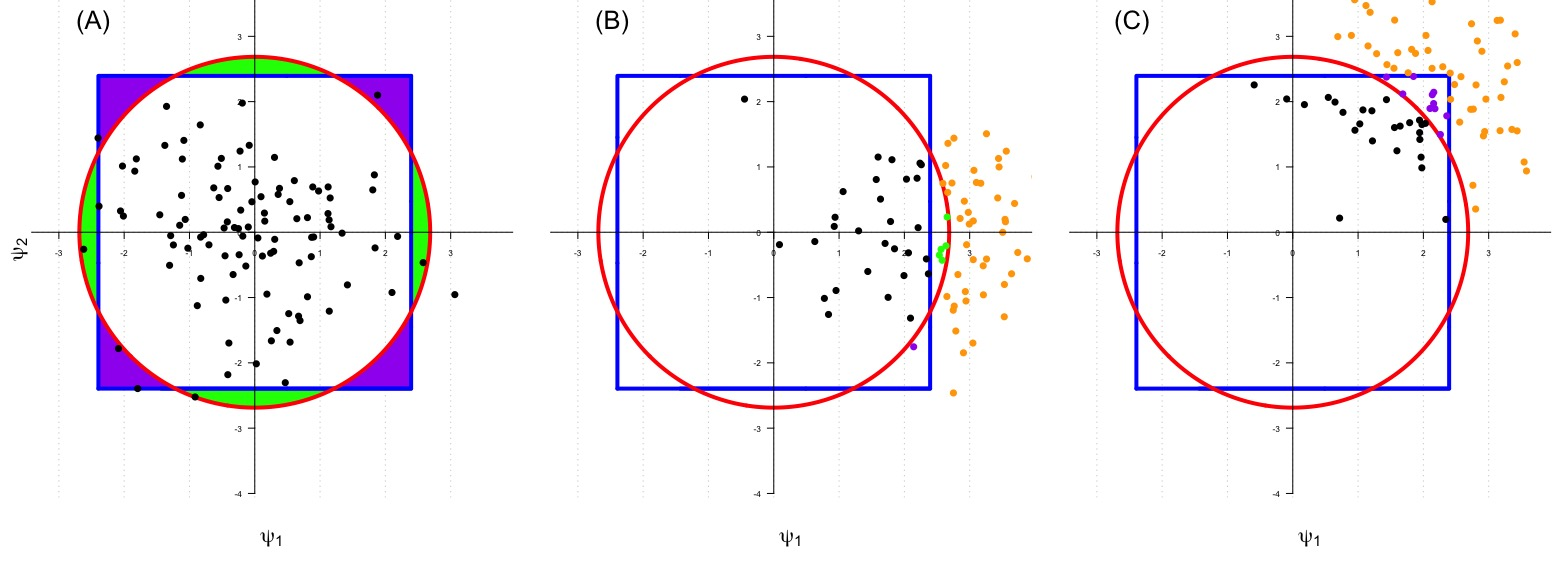
\includegraphics[width = \linewidth]{figure_code/pwr_cmp.jpeg}
	\caption{Plots of 100 observations from a limiting distribution of a hypothetical vector of parameter estimators in $\mathbb{R}^2$ (A) under the null, (B) under an alternative with $\psi_1 = 0, \psi_2 \neq 0$, and (C) under an alternative with $\psi_1, \psi_2 \neq 0$. The 95\% quantiles for the data based on the max (blue) and $\ell_2$ (red) norms under the null are given in all three panels. If a test statistic fell within the purple regions the test would fail to reject $H_0$ if the $\ell_\infty$ norm was used, but would reject $H_0$ if the $\ell_2$ norm was used.  The converse is true for the green regions.  Depending on the alternative, the $\ell_\infty$ norm (B) or the $\ell_2$ norm(C) will achieve higher power.}
	\label{fig:figure1}
\end{figure}

% \subsection{\textcolor{blue}{Creating a rejection region using a function}}
% Note that above while our test was defined by rejecting or accepting based on if $\sqrt{n}\hat{\psi} \in \Theta_0$, we can also think about defining our test decision based on if some function, say $\Gamma_P(x, ||\cdot||)$ that maps from a value and distribution in $\mathbb{R}^d$, and a norm $||\cdot||$ to a real value is greater than zero.

Above we used a norm to constrain the considered rejection regions and allow for a test based on the value of $\sqrt{n}\hat{\boldsymbol{\psi}}$ under the norm the distribution of $\rvv$ under the norm, both of which reside in $\mathbb{R}$.
Above, we have used a single norm to transform both the distribution of $\rvv$ and $\sqrt{n}\hat{\boldsymbol{\psi}}$ into $\mathbb{R}$ which allows for creating tests and calculating p-values similar to the univariate case. 
% \textcolor{blue}{I don't understand the end of this sentence}.
However, this approach also works with more complicated functions.  For every distribution $\distv$ with support conntained in $\mathbb{R}^d$, let $\Gamma_{\distv}$ be a function mapping from  $\mathbb{R}^d$ to $\mathbb{R}$.
% \textcolor{blue}{I see $\Gamma_{\distv}$ being an $\mathbb{R}^d$ to $\mathbb{R}$ function. I don't see $\Gamma_Q(x)$ being a function? I also don't understand how this maps ``from a ... distribution'' to anywhere? Do you mean: ``For any distribution $Q$ with support contained in $\mathbb{R}^d$, let $\Gamma_Q$ be a function mapping from $\mathbb{R}^d$ to $\mathbb{R}$''?}
The distribution of $\Gamma_\distv(\rvv)$ \textcolor{blue}{(when $Z$ is sampled from what?)} can be compared to $\Gamma_\distv(\sqrt{n}\hat{\boldsymbol{\psi}})$ to obtain p-values and define a test. An example of $\Gamma_\distv$ is given below:
% any test defined using an acceptance region can also be carried out using a function, say $\Gamma_\distv(x)$ that maps from a value and distribution in $\mathbb{R}^d$.  Trivially, this function could be defined as: $\Gamma_{\distv(\disto)}(x) = I\{x \in \Theta_0(\disto)\}$.  However, in other cases, (for example the $\ell_2$ ball), this function can be more intuitive and can change depending on the norm.  
% In the previous example, $\Gamma_\distv(x) = Pr_\distv\left(||\rvv|| \geq ||x|| \right)$.  For this definition of $\Gamma$, we knew the distribution of $\Gamma_\distv(\rvv)$ is uniformly distributed on $(0, 1)$.  However, for other $\Gamma$, this may not be the case. Consider 
\begin{align*}
	\Gamma_\distv(x) &= Pr_\distv(||\rvv^* + x|| > c_{0.8})  \text{ where }  c_{0.8} \equiv \min_{c}\{c : Pr_\distv(||\rvv|| < c) \geq 0.8 \} \text{ and } \rvv^* \overset{d}{=} \rvv.
\end{align*}
\textcolor{blue}{What is $\rvv^* \overset{d}{=} \rvv$ telling us? Don't we already know that the probabilities over both of these quantities are indexed by $Q$? Also, why use different notation at all? Why not just $\rvv^*$ for both?}
% In this scenario, the test can be carried out by comparing our test statistic, $\Gamma_\distv(\sqrt{n}\hat{\boldsymbol{\psi}}, ||\cdot||)$ to $\Gamma_\distv(\rvv, ||\cdot||).$

% This test statistic was then compared to the estimated limiting distribution of the test statistic under the null.  The key components of this test were to create a real valued summary of the observed test statistic, and compare this test statistic to draws of the test statistic under the null.  In the previous example, the test statistic was the quantile of the $\ell_2$ norm of our vector of parameter estimates.  We already know the distribution of this statistic is uniform from zero to one under the null, so calculating the p-value is trivial.

% However, we could consider other test statistics.  One example would be the estimated power of an observation is from the $80\%$ quantile of the limiting distribution under the null.  Here, while smaller values indicate more evidence against the null, the distribution of this test statistic is not as straightforward.  While more difficult, the distribution of this test statistic can be be estimated using a bootstrap.  We can take a single observation from our estimated limiting distribution of $\sqrt{n}\hat{\psi}$ and then find its multiplicative distance from the $80\%$ quantile under the $\ell_2$ norm.  This can be done many times to create a limiting distribution of our test statistic.  A p-value can then be obtained by comparing the test statistic to the bootstrapped test statistics.	

While this method for defining tests allows for many different specifications, it often requires choosing a norm as part of the definition of $\Gamma$.  Figure \ref{fig:figure1} shows that the power a test achieves can depend on the norm chosen.  Consider the case when $d = 2$ and $100$ draws are taken from $Z$.  Cutoffs can be obtained by transforming these data (using the $\ell_p$ norm) and taking the 95\% quantile of this transformed data. The perimeter of the acceptance region when using the $\ell_2$ and $\ell_{\infty}$ norm are given in red and blue respectively. If $\sqrt{n}\hat{\boldsymbol{\psi}}$ falls within any of the purple regions, using the $\ell_\infty$ norm would result in failing to reject $H_0$ and using the $\ell_2$ norm would result in rejecting $H_0$.  The converse is true for the green regions.  

\subsection{Adaptive selection of a norm}
In the previous section it was shown that a test can be defined by choosing a summarizing function and norm. However, the choice of norm influences the power of the test. In most scenarios it will not be clear a priori which norm will have maximal power for the true alternative. The procedure proposed in this section adaptively selects a norm and it will be shown that this procedure achieves greater power than a test with a fixed norm, while maintaining type 1 error control.  

To achieve this, first define $\Gamma_{1, \distv}(x), \dots, \Gamma_{p, \distv}(x)$ as collection of functions in which the functions only differ by the norm used in their definition. Next, define
% by defining a $\Gamma$ to those defined earlier, except the optimal norm is selected, and the corresponding summary value of $\Gamma$ with the optimal norm is returned.  For example, if we had $p$ different norms, $\norm_1, \dots, \norm_p$ and some summary function $\Gamma_\distv(x, ||\cdot||)$, we would define the adaptive version of $\Gamma$ as
\begin{align*}
	\Gamma^*_\distv(x) = \max\left\{\Gamma_{1, \distv}(x), \Gamma_{2, \distv}(x), \dots, \Gamma_{p, \distv}(x)\right\}.
\end{align*}
\textcolor{blue}{This could be the min if smaller values indicate larger distances away from the norm (such as p-values).}  

While this function is more complicated than before,  $\Gamma^*_{\distv}(\rvv))$ can still be compared to $\Gamma^*_{\distv}(\sqrt{n}\hat{\psi})$ to obtain a p-value. Also, while it may be difficult to obtain the exact distribution of $\Gamma_\distv^*(\rvv)$, the distribution is a function of $\distv$, so obtaining very good approximations of $\Gamma_\distv^*(\rvv)$ is possible by taking many draws from $\rvv$. This technique can be used both to estimate the function $\Gamma$ and to estimate $\Gamma^*_\distv(\rvv)$ .

% Let $g_1, \dots, g_k$ be a list candiate norms, and let $\boldsymbol{Z}_1, \dots, \boldsymbol{Z}_B$ and $\boldsymbol{V}_1, \dots, \boldsymbol{V}_B$ independent draws from $Q$.  For each of the possible norms, let a p-value be defined using the following quantity:

% \begin{align*}
% s_{p}\left(\sqrt{n}\hat{\boldsymbol{\psi}}, \boldsymbol{Z}_1, \dots, \boldsymbol{Z}_B\right) = \frac{1}{B}\sum_{i=1}^B I\left\{g_p\left(\sqrt{n}\hat{\boldsymbol{\psi}}\right)  \leq g_p(\boldsymbol{Z}_i)\right\}
% \end{align*}

% Using the $c_{p, \alpha}$ defined earlier, it is possible to obtain estimates of power for each norm for any assumed vector of parameters:
% \begin{align*}
% \hat{\omega}_{\alpha, p}(\boldsymbol{h}) = \frac{1}{B} \sum_{i=1}^B I\left\{g_p\left(\boldsymbol{h} + \boldsymbol{V}_i\right) \geq \hat{c}_{\alpha, p}\right\}
% \end{align*}
% The last quantity considered is the multiplicative distance the vector of parameter estimates is from a vector in the same direction which obtains a certain power:
% \begin{align*}
% \hat{r}_{\alpha, p}(a) = \min\left\{r : \hat{\omega}_{\alpha, p}(r \times \sqrt{n}\hat{\boldsymbol{\psi}}) > a\right\}
% \end{align*}
% As described above, there are a multitude of ways to evaluate the performance of the various norms.  Let $f_p(x_1, \dots, x_k)$ be the function that takes the observed data and a norm and returns a measure of the norm's estimated performance given the observed data. $f$ could be $s_p$, $\hat{\omega}_{\alpha, p}$, $\hat{s}_{\alpha, p}$, or some other function.  Let $p^*$ be the index of the ``optimal'' norm.  What is optimal depends on $f$.  If $f$ is the p-value measure $s_p$ then the optimal norm minimizes the $p-value$.  However if instead $f$ is estimated power, then the optimal norm maximizes estimated power.     

% Define the test statistic $\hat{t}$ as 
% \begin{align*}
% \hat{t} = f_{p^*}(\boldsymbol{x}_1, \dots, \boldsymbol{x}_n)
% \end{align*}
% While it is not necessary to do this, the same $f$ used for norm selection will be used to define our test statistic.

\subsection{Obtaining the null distribution}
\label{ssec:obtaining_null}
The above procedure requires knowledge of the limiting distribution of $\sqrt{n}\hat{\boldsymbol{\psi}}$ when $P \in \mathscr{M}_0$.  To obtain an estimate of this limiting distribution, assume the vector of parameter estimates $\hat{\boldsymbol{\psi}}$, converges to a normal distribution with an estimable variance covariance matrix when properly centered and normalized. Also assume each of the estimators $\hat{\boldsymbol{\psi}}_1, \dots, \hat{\boldsymbol{\psi}}_d$ of $\boldsymbol{\psi}_1, \dots, \boldsymbol{\psi}_d$ is asymptotically linear.  That is for each $j \in \{1, \dots, d\}$:
\begin{align*}
\hat{\psi}_j = \psi_j + \frac{1}{n}\sum_{i=1}^n D_j(\boldsymbol{x}_i) + o_p(1/\sqrt{n}) \text{ for some function } D_j
\end{align*}
When there is a fixed number of covariates, the Cramer-Wold device can be used to show that the vector of parameter estimates is asymptotically normal with mean zero, and variance covariance matrix given by $\Sigma = E_{\disto_0}\left[D(\rvo) D(\rvo)^\top \right]$:
%  \textcolor{blue}{Note from Alex: do you mean $D(\rvo) D(\rvo)^\top$? This is what you would want if $D(\rvo)$ were a column vector, which would be more standard (similar comment in other places where `$\top$' is used)}

\begin{align*}
    \sqrt{n}\left(\hat{\boldsymbol{\psi}} - \boldsymbol{\psi}\right) \xrightarrow{d} Z \sim N\left(0, \Sigma\right)
\end{align*}
Under $H_0$, $\sqrt{n}\hat{\boldsymbol{\psi}}$ converges to $Z$, and $\Sigma$ can be approximates with $\widehat{\Sigma} = \frac{1}{n}\sum_{i = 1}^n D(\boldsymbol{x}_i) D(\boldsymbol{x}_i)^\top$.  Thus, in practice we will use an estimate of $\distv$, $\hat{\distv}$ which is distributed $N(0, \widehat{\Sigma})$ in place of $\distv$, and the random variable $\hat{\rvv}$ with distribution $\hat{\distv}$ in place of $\rvv$.  Thus, the test statistic will be $\Gamma_{\hat{\distv}}(\sqrt{n} \hat{\boldsymbol{\psi}})$ and will be compared to $\Gamma_{\hat{\distv}}(\hat{\rvv})$.

\subsection{Using a permutation test for the test statistic}
While the above approach works asymptotically, there can be issues for small sample sizes.  To avoid inflated type one error, a permutation based test can be used.  Here, $\hat{\distv}^\#$ is used to define $\Gamma$, and the test will compare $\Gamma_{\hat{\distv}}(\sqrt{n} \hat{\boldsymbol{\psi}})$ to $\Gamma_{\hat{\distv}}(\rvv^\#)$. To determine $\hat{\distv}^\#$, the $Y$'s from the observed data are permuted before calculating $\widehat \Sigma$.  Draws from $\rvv^\#$ are taken by permuting all of the $Y$'s of the observed data.  \textcolor{blue}{There are a few more complications here that need to be figured out.}

\sh{\subsection{Summary of how simulations are run}}

\section{Simulation Study}
\label{sec:sim_stdy}
\subsection{Correlation}
% A wide variety of simulation settings are considered in this section to show the breath of settings in which the adaptive test can be used.  The first setting considers independent draws from a random vector with mean zero and variance-covariance matrix $\Sigma$.  The measure of association between $Y$ and each covariate will be $\text{Cov}(Y, W_{j})/\text{Var}(W_j)$.  The dimension of the vector, denoted $d$ takes values $10, 50$, and $200$.  The number of correlated covariates will be zero, one, or $0.1, 0.2$, or $0.6$ of all the correlated covariates.  The correlation between each of the covariates will be either $0$ or $0.5$.  The sample sizes considered are $100$ and $500$.   

\sh{
\begin{enumerate}
	\item Two-Phase sampling Scheme of correlation
	\item Marginal structural model example.
\end{enumerate}
All three examples will come with simulation results in the form of figures.  Not sure how many figures to use or what sample size(s) to use.
}

\section{Data Application}

\sh{\begin{enumerate}
	\item Data from Peter Gilbert
\end{enumerate}
}

\section{Discussion}

\section{Appendix}

\subsection{Test Consistency}
\label{sec:test_cnsty}

\begin{theorem}
\label{thm:cnst}
Assume the performance metric of choice is $\hat{r}_{\alpha, p}(a)$, and each the norms $g_a$ considered have the following properties: 
\begin{align}
& \text{for } x \in \mathbb{R}^d, \text{ and } s, l > 0, s \cdot \max({\boldsymbol{x}}) \leq g_a(\boldsymbol{x}) \leq l \cdot d \cdot \max({\boldsymbol{x}}) \label{eqn:nrm_bounds}\\
& \text{for } s \leq 1, l \geq 1, g_a(s \cdot \boldsymbol{x}) \leq g_a(\boldsymbol{x}) \leq g_a(l \cdot \boldsymbol{x}) \label{eqn:linegrowth}
\end{align}
Then for all $P \not \in \mathscr{M}_0$ 
\begin{align*}
	Pr \left(\frac{1}{B}\sum_{k = 1}^B I\left\{\hat{T} \leq \hat{T}_k^{\#}\right\} < 0.05\right) \xrightarrow{p} 1 \text{ as } n \to \infty
\end{align*}
or Equivalently 

\begin{align*}
Pr\left(\hat{T} \leq F^{-1}_{\hat{T}^\#}(0.05)\right) \xrightarrow{p} 1 \text{ as } n \to \infty
\end{align*}
\end{theorem}

\begin{proof}
This proof will consist of three parts.  We will first show that as $n \to \infty, \hat{T}_a^\#$ becomes bounded away from $0$ for any valid norm.  Next we will show $\hat{T}_a$ converges to $0$ in probability for any valid norm.  Last we will show the two previous findings imply theorem \ref{thm:cnst}.

Let $P^\#_{\rvo}$ denote the distribution of the randomly permuted observations.  \sh{Because $Pr(Y^{\#}_i \indep \boldsymbol{W}^\#_{i}) \to 0$, $\boldsymbol{\Psi}(P^\#_{\rvo}) = \boldsymbol{0}$.  Additionally, $\sqrt{n}\left(\hat{\boldsymbol{\psi}}^\# -\boldsymbol{\psi}^\# \right) \xrightarrow{d} Z^\# \sim N\left(\boldsymbol{0}, \Sigma_{\text{perm}}\right)$}.
Define $\hat{T}_a^\# = \min_s\{s : g_a(s \cdot \sqrt{n}\hat{\boldsymbol{\psi}}^\#) \geq C_{0.95, a}^\# \}$ and $C^\#_{0.95, a}$ is $F^{-1}_{Z^\#}(0.95)$.  Since we know that $\psi^\# = \boldsymbol{0}$, it follows that $\sqrt{n}\hat{\boldsymbol{\psi}}^\# \overset{d}{\approx} Z^\#$.

Now, consider:
\begin{align*}
	\pr\left(\hat{T}^\#_a  > \epsilon\right) &= \pr\left(g_a\left(\epsilon \cdot \sqrt{n}\hat{\boldsymbol{\psi}}^\#\right) \leq C_{0.95, a}\right)\\
	& \geq \pr\left(\epsilon \cdot d \cdot  \max\left(\sqrt{n} \hat{\boldsymbol{\psi}}^\# \right)\leq C_{0.95, a}\right)\\
	& = \pr\left( \max\left(\sqrt{n} \hat{\boldsymbol{\psi}}^\# \right)\leq C_{0.95, a}/(\epsilon \cdot d)\right)
\end{align*}
Because $\max\left(\left|\sqrt{n} \hat{\boldsymbol{\psi}}^\#\right|\right)$ converges to a well defined, positive distribution as a result of the continuous mapping theorem, for each constant $c < 1$, we know there exists an $\epsilon_c$ such that $\pr\left(\hat{T}^\#_a  > \epsilon_c\right) \geq c$.  

%From the definition of $C_{0.95, a}^\#$ it follows that $Pr(g_a(\sqrt{n}\hat{\boldsymbol{\psi}}^\#) \leq C^\#_{0.95, a}) \to 0.95$.  For realizations in which $g_a(\sqrt{n}\hat{\boldsymbol{\psi}}^\#) \leq C^\#_{0.95, a}$ it must also be true that $\hat{t}^\# > 1$  from \eqref{eqn:linegrowth}. From the above logic it follows that $Pr(\hat{T}_a^\# > 1) \geq 0.95$ and thus $F^{-1}_{\hat{T}_a^\#}(0.05) \geq 1$ with a probability approaching 1.

Now, shifting our focus to $\hat{T}_a$, under alternatives, $\boldsymbol{\psi} \neq \boldsymbol{0}$. Define $\psi_{\max} = \max(\psi_1, \dots, \psi_d)$.  Using this knowledge, and \eqref{eqn:nrm_bounds}, note that 
\begin{align}
\pr\left(\hat{T}_a < \epsilon\right) &= \pr\left(g_a\left(\epsilon \cdot \sqrt{n} \hat{\boldsymbol{\psi}}\right) \geq C_{0.95, a}\right) \nonumber\\
&\geq \pr\left(\epsilon \cdot \sqrt{n}\max(\hat{\psi}_1, \dots, \hat{\psi}_d) \geq C_{0.95, a}\right) \nonumber \\
&= \pr\left(\max(\hat{\psi}_1, \dots, \hat{\psi}_d) \geq C_{0.95, a}/\left(\epsilon \cdot \sqrt{n}\right)\right) \nonumber \\
&\geq \pr\left(\max(\hat{\psi}_1, \dots, \hat{\psi}_d) \geq \psi_{\max}/2\right) \pr\left(\psi_{\max}/2\geq C_{0.95, a}/\left(\epsilon \cdot \sqrt{n}\right)\right) \label{eqn:prod_tlte} 
\end{align}
The first factor of the product in \eqref{eqn:prod_tlte} will converge to 1 as $n \to \infty$ from the consistency of $\hat{\boldsymbol{\psi}}$.  The second quantity will be equal to 1 for sufficiently large $n$.   Thus $\hat{T}_a \xrightarrow{p} 0$ under any alternative.   

It was shown that for each $a$ that $\hat{T}_a \xrightarrow{p} 0$.  This means that our adaptive estimator $\hat{T} \xrightarrow{p} 0$ as well.  Now, let $c = 0.05/k$ and $\epsilon_c$ be small enough that $\pr\left(\hat{T}^\#_a  > \epsilon_c\right) \geq 1 - (0.05/k)$.  The permutation version of the adaptive estimator $\hat{T}^\#$ has the property that
\begin{align*}
	\pr\left(\hat{T}^\# < \epsilon_c\right) \leq \pr(\hat{T}^\#_1 < \epsilon_c) + \dots + \pr(\hat{T}^\#_k < \epsilon_c) \leq 0.05,
\end{align*}
and the theorem's conclusion follows.
\end{proof}

\sh{\subsection{Unbiasedness at local alternatives}
Show that the test will reject the null with a probability greater than $\alpha$ for an $\alpha$ level test }
\sh{Proof Outline: \\
\begin{itemize}
	\item Under local alternatives, $\sqrt{n}\hat{\boldsymbol{\psi}} \xrightarrow{d} N(\boldsymbol{c}, \Sigma)$
	\item The permutation test statistic will converge in distribution to a standard normal.  This paper should help: \citep{omelka_testing_2012}
	\item For each norm selected, \citep{gupta_inequalitites_1972} states that the power will be non-decreasing as long as the rejection region is convex (This should be true most of our rejection regions), and the probability density is decreasing away from the mean (which is true of a normal distribution).  
	\item Show that for $n$ large, the norm is selected to give the best power.  Thus since each norm obtains local power, the adaptive test will also obtain local power for $n$ large.
\end{itemize}} 

\sh{\subsection{Consistency of norm selection} 
This proof would likely be difficult and require some slower than $\sqrt{n}$ covergence rates of the local alternative considered.  Under fixed alternatives, all norms perform equally perfectly}

\sh{\subsection{Type 1 error control}
Proof is so short, I am not sure if it is worth including
Under the null, $Y \indep \rvo$.  Thus the test statistic will be taken from the same distribution as all of the permutation based test statistics used to estimate the distirbution of the test statistic under the null.  Therefore, as $B$ grows, $Pr(T_n \geq F_{T^\#_{k,n}|\rvo_n}(0.95)) \Rightarrow 0.05$
}

%However, determining which observations should be considered more extreme is not straightforward.  
%One way to solve this problem is by using a norm to transform all of your data to $\mathbb{R}$ instead of $\mathbb{R}^d$.  After taking the norm of your vector of parameter estimates and your estimated limiting distribution you can create a cutoff for your test.
% People are interested in discovering if their data about $\rvo$ could be predictive of some outcome $Y$.  While many there have been many procedures that have come before this one, the procedure outlined in this article has a few distinct advantages that are valuable to scientists.  

% For each covariate of interest, we can specify a measure of association between the covariate of interest and the outcome which is defined as a parameter of the data generating mechanism.  This measure of association can be estimated for each covariate of interest giving us a parameter for each covariate of interest. The null hypothesis which we will be testing is whether or not all of these parameters are equal to zero (or some other value which indicates no association exists).

% As with most test, our test will calculate a test statistic, and then estimate the limiting distribution of this test statistic under the null. Obtaining the test statistic is a three step procedure.  The first step is to obtain the limiting distribution of the vector of parameter estimates under the null.  This first step is made possible through the use of influence functions and a multiplier bootstrap.  This technique is applicable for a wide range of parameters that measure association.  Next, a norm is selected from a range of possible norms based on the norms' approximated performance under various alternatives.  After this, the selected norm is applied to the vector of parameter estimates and transformed by a function (which could be dependent on the norm) to give us our test statistic.  

% There are two options for obtaining the limiting distribution of this test statistic under the null.  The first is to use a parametric bootstrap.  We can take a single draw from the limiting distribution of our vector of parameter estimates under the null and treat this draw as if it were our vector of parameter estimates.  Using the same three step procedure described above we can obtain a single draw from the limiting distribution of our test statistic under the null.  This procedure can be repeated many times over to obtain the limiting distribution of our test statistic under the null.  The other option is to randomly permute our outcome variable and use this data to estimate the vector of parameter estimates.  Passing this vector through the three step procedure, we obtain a draw from the limiting distribution under the null.  Many draws can be obtained by taking many draws coming from different permutations of the outcome variable.  

% The permutation technique is less prone to inflated type 1 error rates, but comes at the cost of larger computational burden.

% The procedure is fast because estimation of the limiting distribution is done using a multiplier bootstrap.  The procedure's use of influence functions allows scientists to define the parameter of association that is best suited to answering their scientific question.  Adaptive selection of the norm used improves the testing procedure's ability to detect an association when one exists for a wide variety of data generating mechanisms.  Simulating the test-statistic generating procedure under the null using a permutation guarantees family-wise error control. 
\bibliography{paper_bib}

\end{document}
